\documentclass{beamer}
\usepackage[utf8]{inputenc}
\usepackage{amsmath}
\usepackage{amssymb}
\usepackage{graphicx}
\usepackage[linesnumbered,ruled,vlined]{algorithm2e}
\usepackage{tikz}
\usetikzlibrary{shapes.geometric, arrows, backgrounds, calc}
\usetikzlibrary{shapes, positioning, circuits.ee.IEC}
\usepackage{qrcode}
\usepackage{booktabs}
\usepackage{multirow}
\usepackage{ragged2e}

% Tema da apresentação
\usetheme{CambridgeUS}

% Pacote de cores
\usecolortheme{seahorse}

% Definir paleta de cores
\definecolor{techblue}{RGB}{0, 102, 204}
\definecolor{techgreen}{RGB}{34, 153, 84}
\definecolor{techgray}{RGB}{240, 240, 240}
\definecolor{codebg}{RGB}{30, 30, 30}
\definecolor{techred}{RGB}{204, 0, 0}
\definecolor{techyellow}{RGB}{204, 204, 0}

% Personalizar estilo dos títulos e subtítulos
\setbeamercolor{frametitle}{bg=techblue, fg=white}
\setbeamercolor{title}{fg=techgreen}
\setbeamerfont{frametitle}{series=\bfseries, family=\sffamily}
\setbeamerfont{title}{series=\bfseries, family=\sffamily}

\title{Robótica Probabilística }
\subtitle{Jefferson Bezerra dos Santos}
\author{}
\date{}

\begin{document}

\begin{frame}{Robótica Probabilística}
    \titlepage
    
    \vspace{-2.2cm}
    
    \begin{columns}
        \begin{column}{0.5\textwidth}
            \centering
            \includegraphics[width=0.85\textwidth, height=4.0cm]{introducaoImage.jpg}
        \end{column}
        
        \begin{column}{0.5\textwidth}
            \begin{block}{\textbf{\large Pilares Fundamentais}}
                \begin{itemize}
                    \item \textbf{Modelagem} de incertezas sensoriais
                    \item \textbf{Estimativa} de estado (filtros bayesianos)
                    \item \textbf{Classificadores} atualização do estado
                    \item \textbf{Decisão} sob incerteza
                \end{itemize}
            \end{block}
             
        \end{column}
    \end{columns}
\end{frame}

\section{Justificativa}

\begin{frame}{Justificativa}
    \begin{block}{Problema}
        Robôs autônomos operam em ambientes reais caracterizados por:
        \begin{itemize}
            \item Incerteza sensorial (ruído, imprecisão)
            \item Incerteza de atuação (derrapagem, imprecisão motora)
            \item Ambientes dinâmicos e imprevisíveis
        \end{itemize}
    \end{block}
    
    \begin{block}{Solução Proposta}
        Abordagens probabilísticas oferecem:
        \begin{itemize}
            \item Framework matemático rigoroso para lidar com incertezas
            \item Estimativas de confiança para decisões
            \item Robustez em ambientes complexos
            \item Implementação eficiente em hardware limitado
        \end{itemize}
    \end{block}
\end{frame}

\section{Revisão da Literatura}

\begin{frame}{Revisão da Literatura}
    \begin{columns}[T]
        \begin{column}{0.48\textwidth}
            \begin{block}{\textbf{Fundamentos Teóricos}}
                
                \begin{itemize}
                    \item \textcolor{blue}{\textbf{Teorema de Bayes}} \\
                    \scriptsize Atualização de crenças
                    
                    \item \textcolor{blue}{\textbf{Filtros Bayesianos}} \\
                    \scriptsize Thrun (2005)
                    
                    \item \textcolor{blue}{\textbf{Classificadores}} \\
                    \scriptsize Naive Bayes \\
                    \scriptsize Redes Bayesianas
                \end{itemize}
            \end{block}
        \end{column}
        
        \begin{column}{0.48\textwidth}
            \begin{block}{\textbf{Principais Contribuições}}
                
                \begin{itemize}
                    \item \textbf{Thrun et al. (2005)} \\
                    \scriptsize \textit{Probabilistic Robotics}
                    
                    \item \textbf{Montemerlo et al. (2002)} \\
                    \scriptsize Filtro de partículas - \textit{Stanley}
                    
                    \item \textbf{Dellaert et al. (1999)} \\
                    \scriptsize FastSLAM
                    
                    \item \textbf{Fox et al. (1999)} \\
                    \scriptsize Amostragem adaptativa
                \end{itemize}
            \end{block}
        \end{column}
    \end{columns}

    \vspace{0.3cm}
    
    \centering
    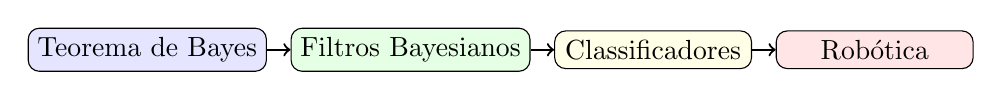
\begin{tikzpicture}[node distance=0.3cm]
        \node[draw, fill=blue!10, rounded corners, minimum width=2.5cm] (bayes) {Teorema de Bayes};
        \node[draw, fill=green!10, rounded corners, minimum width=2.5cm, right=of bayes] (filters) {Filtros Bayesianos};
        \node[draw, fill=yellow!10, rounded corners, minimum width=2.5cm, right=of filters] (applications) {Classificadores};
        \node[draw, fill=red!10, rounded corners, minimum width=2.5cm, right=of applications] (robotics) {Robótica};
        
        \draw[->, thick] (bayes) -- (filters);
        \draw[->, thick] (filters) -- (applications);
        \draw[->, thick] (applications) -- (robotics);
    \end{tikzpicture}
\end{frame}


\section{Objetivos}

\section{Objetivos}

\begin{frame}{Objetivos}
    \centering
    \vspace{-0.3cm}
    
    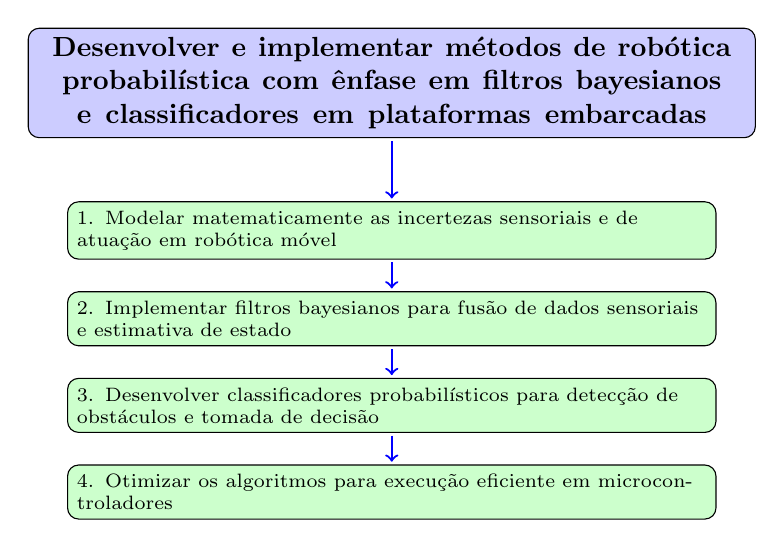
\begin{tikzpicture}[
        node distance=0.4cm,
        objetivoGeral/.style={draw, fill=blue!20, rounded corners, text width=9cm, align=center, minimum height=1cm, font=\normalsize\bfseries},
        objetivoEspecifico/.style={draw, fill=green!20, rounded corners, text width=8cm, align=left, minimum height=0.6cm, font=\scriptsize},
        linha/.style={->, thick, blue, shorten >=1pt, shorten <=1pt}
    ]
    
    % Objetivo Geral (Topo)
    \node[objetivoGeral] (geral) {
        \justifying
        Desenvolver e implementar métodos de robótica probabilística com ênfase em filtros bayesianos e classificadores em plataformas embarcadas
    };
    
    % Objetivos Específicos (Lista vertical)
    \node[objetivoEspecifico, below=of geral, yshift=-0.4cm] (oe1) {
        1. Modelar matematicamente as incertezas sensoriais e de atuação em robótica móvel
    };
    
    \node[objetivoEspecifico, below=of oe1] (oe2) {
        2. Implementar filtros bayesianos para fusão de dados sensoriais e estimativa de estado
    };
    
    \node[objetivoEspecifico, below=of oe2] (oe3) {
        3. Desenvolver classificadores probabilísticos para detecção de obstáculos e tomada de decisão
    };
    
    \node[objetivoEspecifico, below=of oe3] (oe4) {
        4. Otimizar os algoritmos para execução eficiente em microcontroladores
    };
    
    % Conexões verticais
    \draw[linha] (geral.south) -- (oe1.north);
    \draw[linha] (oe1.south) -- (oe2.north);
    \draw[linha] (oe2.south) -- (oe3.north);
    \draw[linha] (oe3.south) -- (oe4.north);
    
    \end{tikzpicture}
    
\end{frame}

\section{Metodologia}

\begin{frame}{Metodologia: Filtros e Classificadores Bayesianos}
\scriptsize  % reduz toda a fonte do slide, incluindo fórmulas

    \begin{columns}[t]  % alinha o topo das colunas
        % Coluna da esquerda: Filtro Bayesiano
        \column{0.48\textwidth}
        \begin{block}{Filtro Bayesiano}
            \textbf{Predição:}
            \[
                \overline{bel}(x_t) = \int p(x_t | u_t, x_{t-1}) \, bel(x_{t-1}) \, dx_{t-1}
            \]
            \textbf{Correção:}
            \[
                bel(x_t) = \eta \, p(z_t | x_t) \, \overline{bel}(x_t)
            \]
            \begin{itemize}\scriptsize
                \item $bel(x_t)$: crença no estado
                \item $u_t$: ação de controle
                \item $z_t$: medida do sensor
                \item $\eta$: fator de normalização
            \end{itemize}
        \end{block}

        % Coluna da direita: Naive Bayes
        \column{0.48\textwidth}
        \begin{block}{Naive Bayes}
            \textbf{Fórmula:}
            \[
                P(C_k | \mathbf{x}) \propto P(C_k) \prod_{i=1}^{n} P(x_i | C_k)
            \]
            \begin{itemize}\scriptsize
                \item $\mathbf{x}$: medições dos sensores
                \item $C_k$: classe/estado (ex.: obstáculo)
                \item $P(C_k)$: probabilidade a priori
                \item $P(x_i|C_k)$: probabilidade condicional
                \item $\prod$: produto das condições
            \end{itemize}
            \textbf{Exemplo:}
            \[
                P(\text{obstáculo}|d) = \frac{P(d|\text{obstáculo}) P(\text{obstáculo})}{P(d)}
            \]
        \end{block}
    \end{columns}

\end{frame}


\section{Referências}

\begin{frame}{Referências}
    \footnotesize
    \begin{thebibliography}{99}
        \bibitem{thrun2005probabilistic}
        THRUN, Sebastian; BURGARD, Wolfram; FOX, Dieter. \textit{Probabilistic Robotics}. MIT Press, 2005.
        
        \bibitem{barber2012bayesian}
        BARBER, David. \textit{Bayesian Reasoning and Machine Learning}. Cambridge University Press, 2012.
        
        \bibitem{särkkä2013bayesian}
        SÄRKKÄ, Simo. \textit{Bayesian Filtering and Smoothing}. Cambridge University Press, 2013.
        
        \bibitem{doucet2001sequential}
        DOUCET, Arnaud; FREITAS, Nando de; GORDON, Neil (Eds.). \textit{Sequential Monte Carlo Methods in Practice}. Springer, 2001.
        
        \bibitem{bishop2006pattern}
        BISHOP, Christopher M. \textit{Pattern Recognition and Machine Learning}. Springer, 2006.
        
        \bibitem{lewis1998naive}
        LEWIS, David D. \textit{Naive (Bayes) at Forty: The Independence Assumption in Information Retrieval}. ECML, 1998.
        
        \bibitem{montemerlo2002fastslam}
        MONTEMERLO, Michael et al. \textit{FastSLAM: A Factored Solution to the Simultaneous Localization and Mapping Problem}. AAAI, 2002.
        
        \bibitem{fox1999monte}
        FOX, Dieter et al. \textit{Monte Carlo Localization: Efficient Position Estimation for Mobile Robots}. AAAI, 1999.
    \end{thebibliography}
\end{frame}

\end{document}
